\documentclass[10pt,a4paper]{article}
\usepackage[utf8]{inputenc}
\usepackage{amsmath}
\usepackage{amsfonts}
\usepackage{amssymb}
\usepackage{graphicx}
\usepackage{subfigure}
\usepackage{amsmath}
\usepackage{mathrsfs}
\DeclareRobustCommand{\orderof}{\ensuremath{\mathcal{O}}}
\bibliographystyle{prsty}
\usepackage[top=1in, bottom=1in, left=1in, right=1in]{geometry}

\begin{document}
\section{Introduction}
\textbf{flq} is a task in application level. It generates the Floquet Hamiltonian\footnote{For detail formulation of Floquet theory, see PRB 88, 245422 (2013) and PRL110,200403 (2013)} Note that, the example attached in this file uses Haldane\_flq.plb instead because NiO is not a good system to have Floquet effects.

\section{Dictionary}

\subsection{Input}
\textit{\textbf{flq.Frequency}} This parameter gives the floquet frequency. \\ \\
\textit{\textbf{flq.Order}} This parameter gives the order of photon process. \\ \\
\textit{\textbf{flq.Amplitude}} This parameter gives the amplitude of the x, y and z direction, e.g [1,1,1]. The periodic wave vector is assume to have the form: $A=[A_{x}*sin(\omega t+\phi_{x}),A_{x}*sin(\omega t+\phi_{y}),A_{x}*sin(\omega t+\phi_{z})]$, this parameters is essentially $[A_{x}, A_{y}, A_{z}]$. \\ \\
\textit{\textbf{flq.Amplitude}} This parameter gives the phase of each components, $[\phi_{x}, \phi_{y}, \phi_{z}]$ in unit of radian. \\ \\ 

\subsection{Output}
\textit{\textbf{flq.state\_info}} This variable shows the Flqouet states used in the calculation. There are 6 column in this variable [state\_label, order, site, identifier, l, SubOrb]. They have similar meaning as shown in the hop.state\_info. The only difference is there is an additional column which shows the ``order''. Since all Floquet states come with an additional quantum number which describes the Fourier component of time domain. Usually we call this quantum number as ``order" because it relates to the number of photons involved. \\ \\
\textit{\textbf{flq.H\_onsite(n)}} This variable shows the onsite energy of Floquet Hamiltonian. Like the Floquet state, the Hamiltonians also requires an additional quantum number to label them, so flq.H\_onsite(n) describes the onsite energy of the (n-1)-th order. \\ \\
\textit{\textbf{flq.hop\_size}} This variable shows the size of the variable flq.hop\_mat. This is just for PiLab to preset memory and most users can ignore this variable. \\ \\
\textit{\textbf{flq.hop\_mat(p)(n)(:,:,m)}} This variable shows the hopping between the n-th sublattice and its m-th neighbor as shown in the hop.hop\_mat. Also, there is an additional variable p to describe the order of the Floquet Hamiltonian.  \\ \\


\begin{figure}[tbp]
\centering
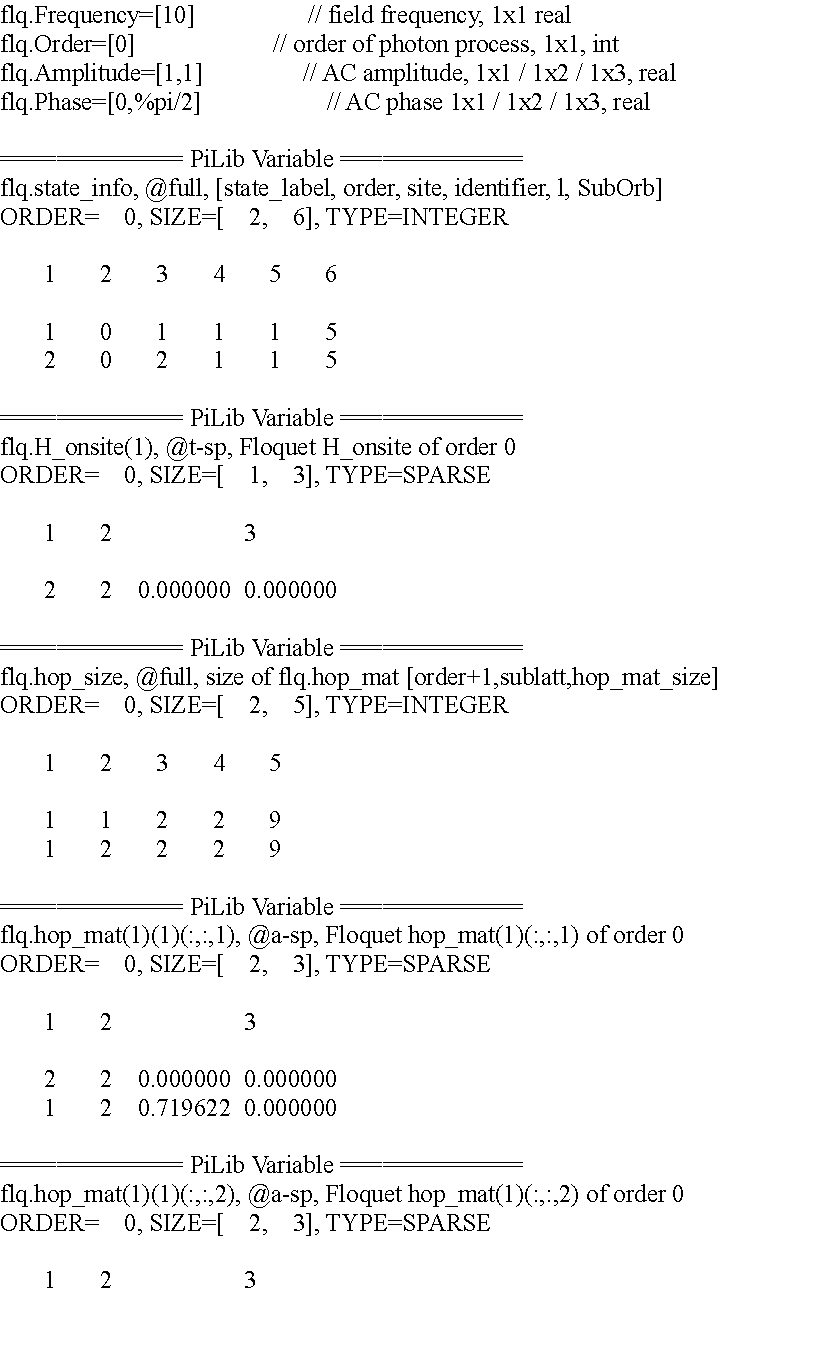
\includegraphics[width=0.85\columnwidth]{Haldane_flq_p1.pdf}
\caption{page 1 of Haldane\_flq.plb}
\end{figure}

\begin{figure}[tbp]
\centering
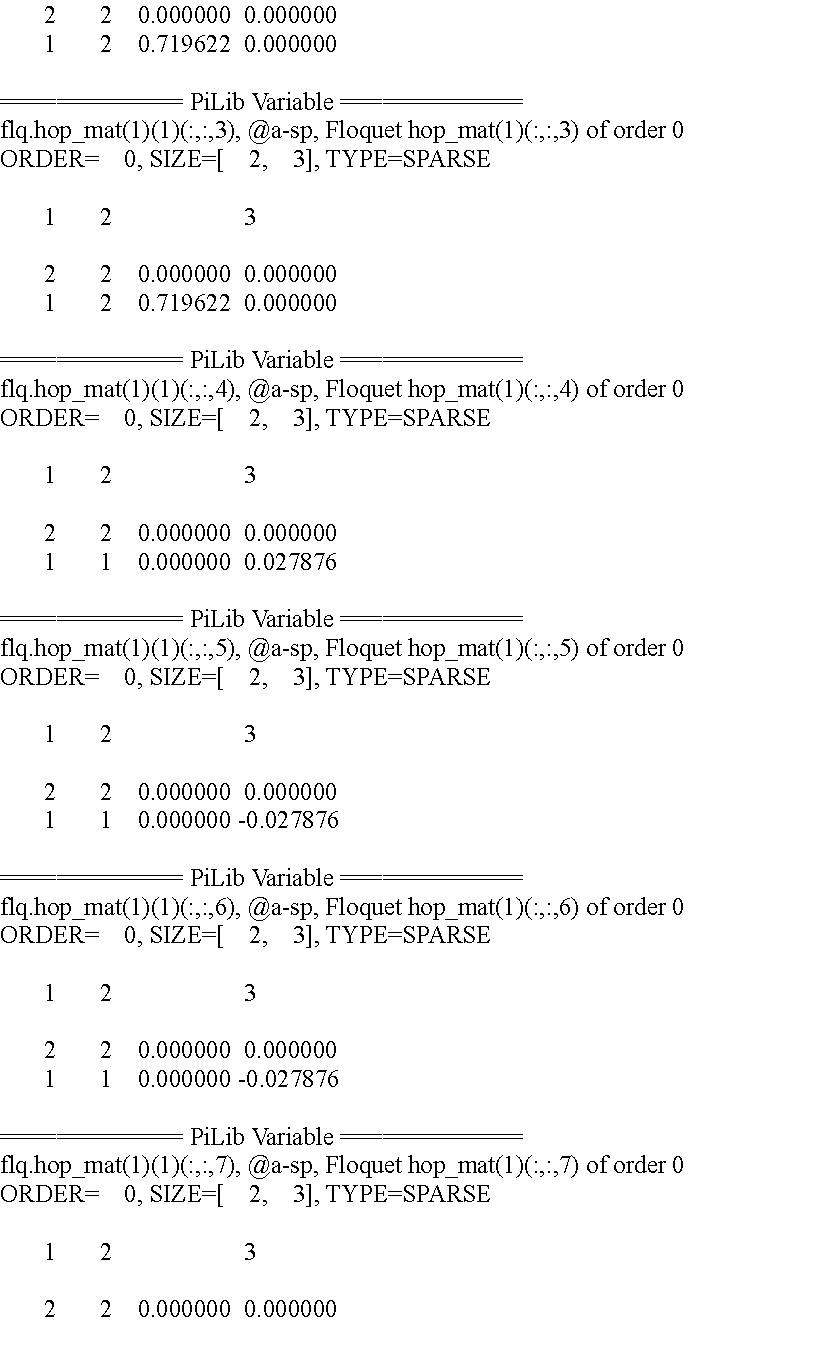
\includegraphics[width=0.85\columnwidth]{Haldane_flq_p2.pdf}
\caption{page 2 of Haldane\_flq.plb}
\end{figure}

\begin{figure}[tbp]
\centering
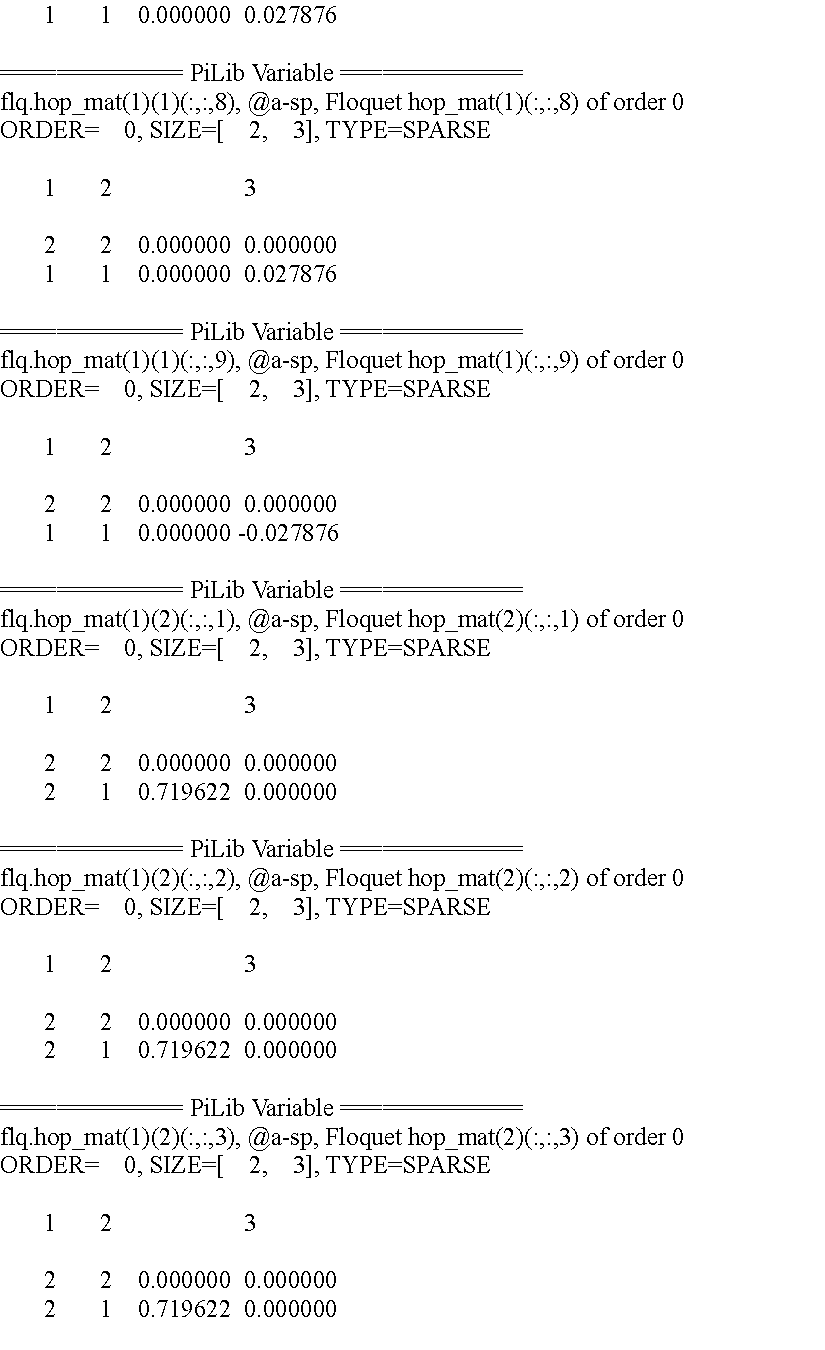
\includegraphics[width=0.85\columnwidth]{Haldane_flq_p3.pdf}
\caption{page 3 of Haldane\_flq.plb}
\end{figure}

\begin{figure}[tbp]
\centering
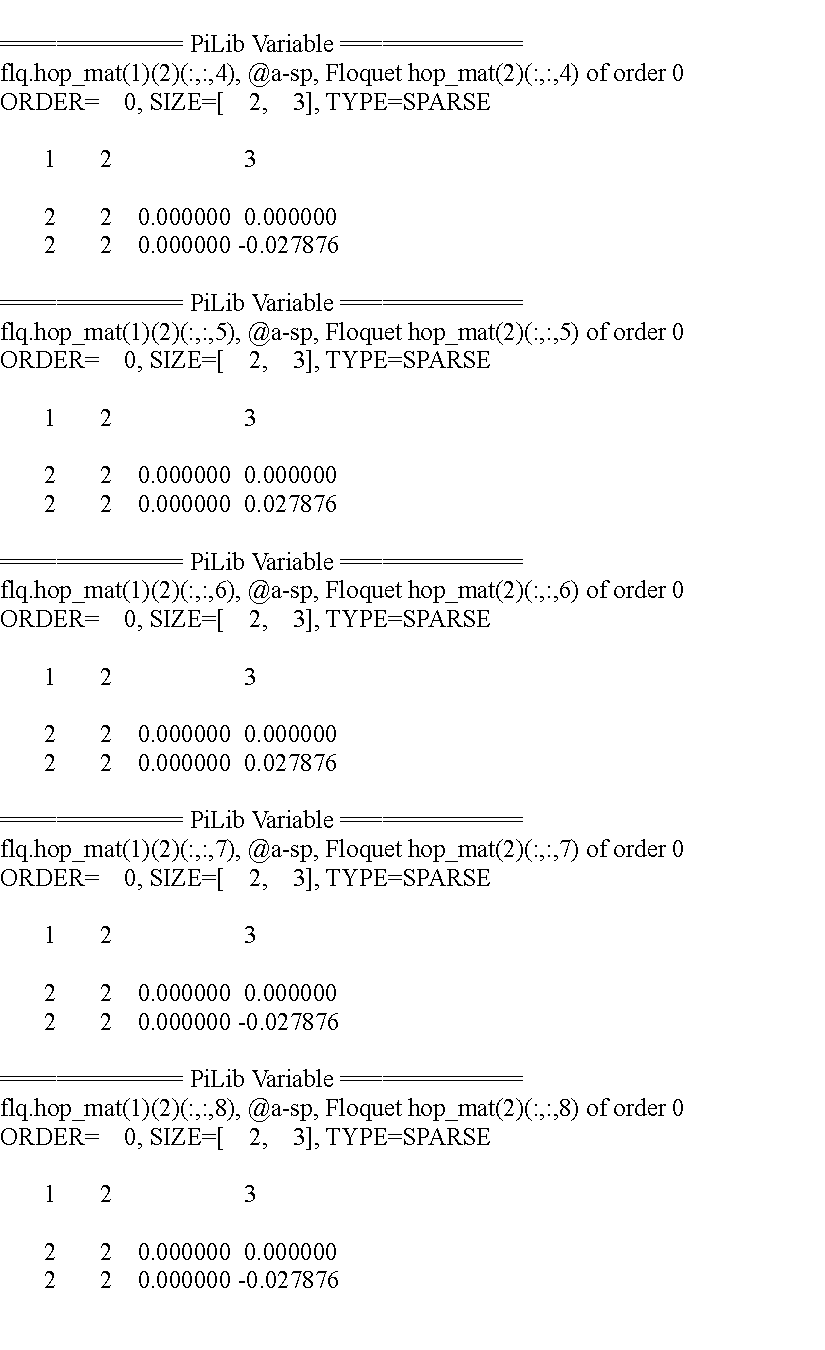
\includegraphics[width=0.85\columnwidth]{Haldane_flq_p4.pdf}
\caption{page 4 of Haldane\_flq.plb}
\end{figure}

\begin{figure}[tbp]
\centering
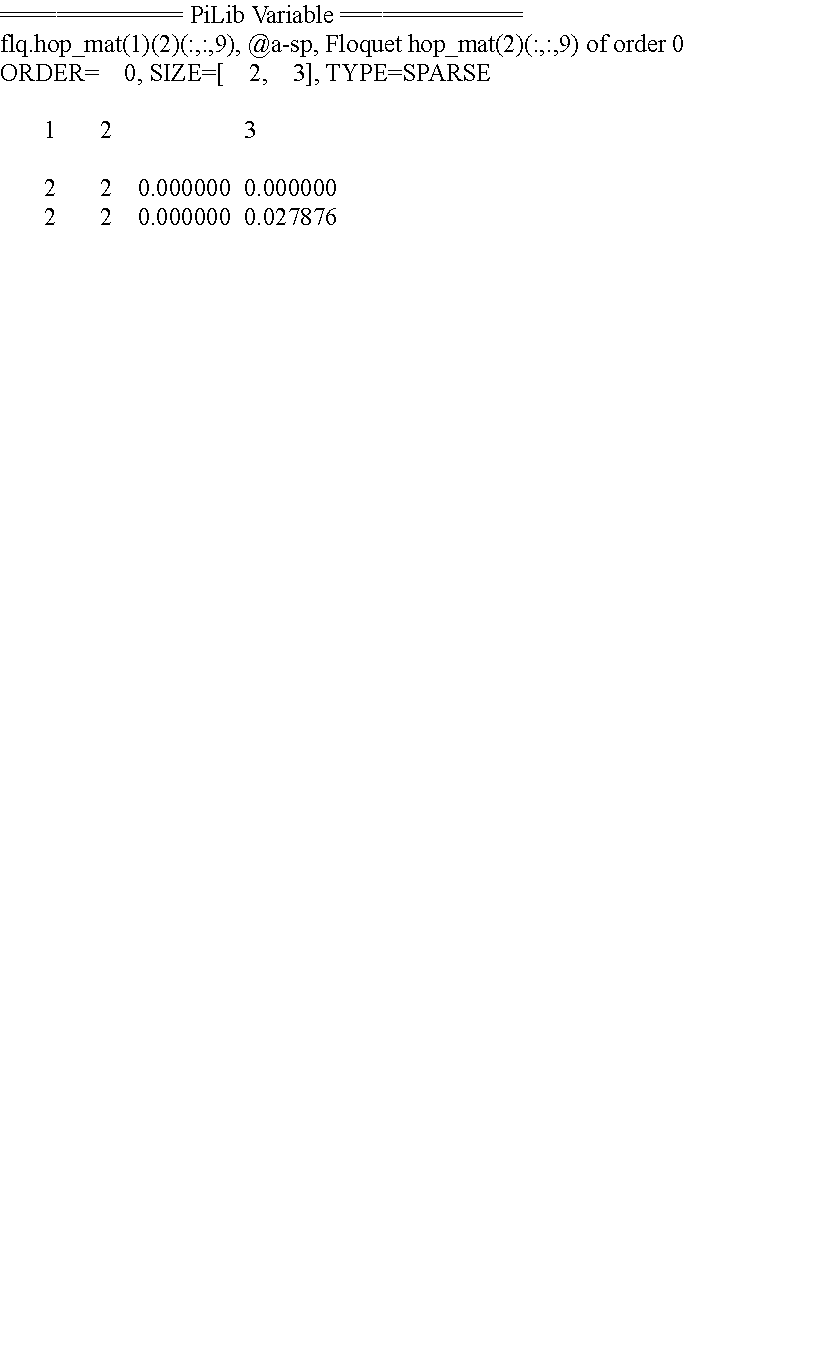
\includegraphics[width=0.85\columnwidth]{Haldane_flq_p5.pdf}
\caption{page 5 of Haldane\_flq.plb}
\end{figure}
\end{document}